\part{Structure du projet}
\chapter{Aspect général}
Le robot a pour objectif de pouvoir déplacer des objets cylindriques (cylindres en bois, et gobelets en plastique). Pour cela, nous l'avons équipé d'une pince adaptée capable de monter et descendre.


\begin{figure}[h]
	\centering

	\begin{floatrow}
		\ffigbox[\FBwidth]{\caption{CAO du robot}}{%
			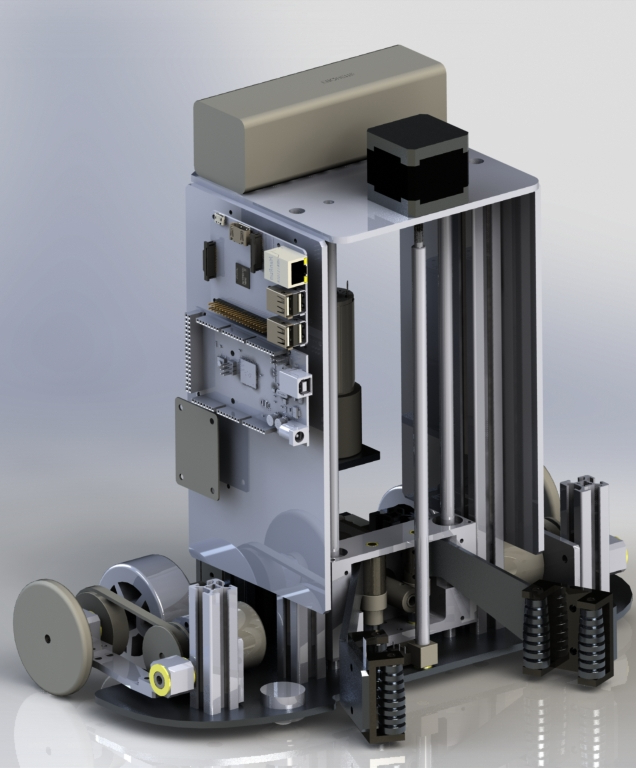
\includegraphics[width=70mm]{assets/3D-robot.jpg}%
		}
		\ffigbox[\FBwidth]{\caption{Photo du robot}}{%
			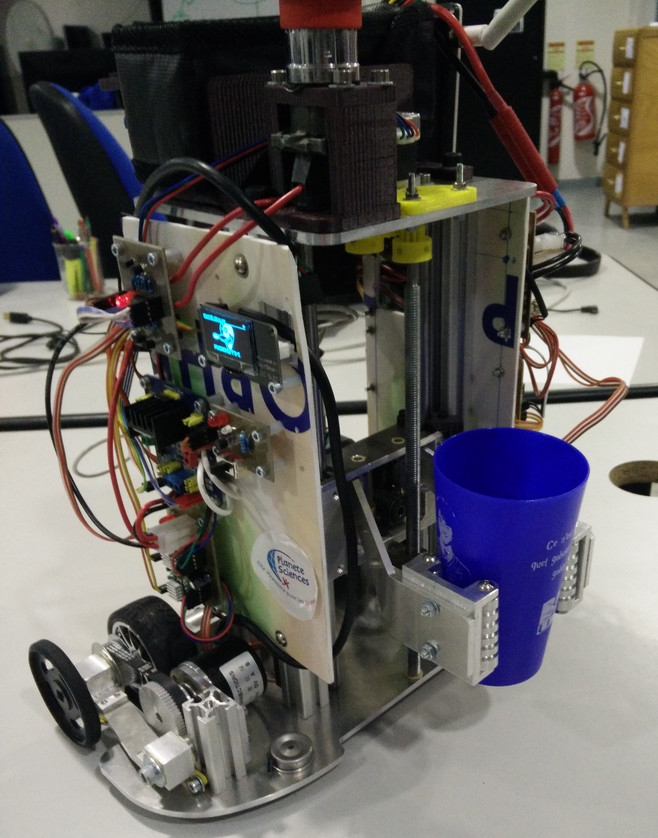
\includegraphics[width=70mm]{assets/photo-robot.jpg}%
		}
    \end{floatrow}
\end{figure}


\newpage
\section{Modularité}
Comme le club participe tous les ans à la coupe de France de Robotique, il y a des actions parfois similaires et certaines parties des robots qui pourraient être réutilisées. C'est en partant de ce constat que nous avons conçu une architecture modulaire. Certains modules pouvant être réutilisés et améliorés les années suivantes. \\


Cette année le robot a donc été séparé en 4 modules :

\begin{itemize}
	\item Coeur
	\item Moteur
	\item Pince 
	\item Capteur
\end{itemize}


\begin{figure}[h]
	\centering
	
% Define block styles
\tikzstyle{module} = [draw, text centered,text width=4em, minimum width=4em,
  minimum height=3.5em,ellipse]
\tikzstyle{object} = [draw, text centered, minimum width=2em,
  minimum height=1.5em]
\tikzstyle{arrow} = [thick, color=black!50, arrows=->, >=latex]
\tikzstyle{texto} = [above, text width=6em, text centered]

\begin{tikzpicture}[scale=0.675,transform shape]

%Modules
\node[module](A1) at (0,2){Coeur};
\node[module](A2) at (3,0){Module Pince};
\node[module](A3) at (0,-2){Module Capteur};
\node[module](A4) at (-3,0){Module Moteur};

%Bus I2C
\draw[arrow, <->] (A1.south) -- (A2.west);
\draw[arrow, <->] (A2.west) -- (A3.north);
\draw[arrow, <->] (A3.north) -- (A4.east);
\draw[arrow, <->] (A4.east) -- (A1.south);
\node[texto] at (0,-1.5ex){$I^2C$ Bus};

%Enfants de coeur
\node[object](B1) at (-2,3.5){Écran};
\node[object](B2) at (0,4.5){Sélection de couleur};
\node[object](B3) at (2,3.5){Lanceur};

\draw[arrow, ->] (A1.100) -- (B1.east);
\draw[arrow, <-] (A1.north) -- (B2.south);
\draw[arrow, <-] (A1.80) -- (B3.west);

%Enfant de moteur
\node[object, rounded corners](C1) at (-8.5,0.5){Contrôleur moteur à courant continu};
\node[object, rounded corners](C2) at (-8.5,-0.5){Carte acquisition roues codeuses};

\draw[arrow, ->] (A4.-190) -- (C1.east);
\draw[arrow, <-] (A4.-170) -- (C2.east);

	%Enfant de Controleur CC
	\node[object](D1) at (-10.25,2){Moteur gauche};
	\node[object](D2) at (-6.75,2){Moteur droit};
	
	\draw[arrow, ->] (C1.120) -- (D1.south);
	\draw[arrow, ->] (C1.100) -- (D2.south);

	%Enfant de acquisition roues codeuses
	\node[object](E1) at (-11,-2){Roue codeuse gauche};
	\node[object](E2) at (-6.75,-2){Roue codeuse droit};
	
	\draw[arrow, <-] (C2.-120) -- (E1.north);
	\draw[arrow, <-] (C2.-100) -- (E2.north);


%Enfants de Cpateur
\node[object](F1) at (-2.5,-3.25){Sonar 1};
\node[object](F2) at (-1,-4){Sonar 2};
\node[object](F3) at (1,-4){Sonar 3};
\node[object](F4) at (2.5,-3.25){Sonar 4};

\draw[arrow, <-] (A3.-120) -- (F1.east);
\draw[arrow, <-] (A3.-100) -- (F2.north);
\draw[arrow, <-] (A3.-80) -- (F3.north);
\draw[arrow, <-] (A3.-60) -- (F4.west);

%Enfant de pince
\node[object, rounded corners](G1) at (8,1){Contrôleur moteur pas à pas};
\node[object](G2) at (8,0){Capteur de fin d'ouverture};
\node[object](G3) at (8,-1){Capteur de fin d'ascension};

\draw[arrow, ->] (A2.20) -- (G1.west);
\draw[arrow, <-] (A2.0) -- (G2.west);
\draw[arrow, <-] (A2.-20) -- (G3.west);

	%Enfant de controleur de moteur pas à pas
	\node[object](G2) at (6,2.5){Moteur ascenseur};
	\node[object](G3) at (10,2.5){Moteur pince};

	\draw[arrow, ->] (G1.110) -- (G2.south);
	\draw[arrow, ->] (G1.70) -- (G3.south);

\end{tikzpicture}

	\caption{Structure des différents modules}
\end{figure}

\section{Programmes et documentation}
Afin de pouvoir travailler à plusieurs sur les programmes, nous utilisons \textit{Git}. C'est un logiciel qui est fait pour pouvoir fusionner des modifications sur les différents fichiers du projet tout en gardant un historique de toutes les modifications. Pour que ce logiciel fonctionne, il faut qu'il y ait un serveur qui stocke tous les codes sources ainsi que l'historique de modification sur Internet.\\

Nous utilisons Github.com, qui est l'un des plus utilisés. Nous avons choisi de ne pas mettre notre code source en publique, car nous participons à une competition. Le fait de mettre en privé du code est payant sur Github.com, cependant nous avons fait la demande à Github d'accorder gratuitement des dépôts\footnote{dépôt: Sorte de dossier où le code d'un projet y est placé}  privés gratuits en tant qu'association étudiante. Ils ont mis deux mois pour étudier la demande avant de l'accepter.\\

\newpage

Les programmes qui font fonctionner le robot suivent l'architecture modulaire. Nous avons donc créé les dépôts suivants :\\
\begin{itemize}
	\item \textit{eurobot-core} : Le code du module Coeur
	\item \textit{eurobot-clampController} : Le code du module Pince
	\item \textit{eurobot-sensorController} : Le code du module Capteur
	\item \textit{eurobot-motorController} : Le code du module Moteur
	\item \textit{eurobot-CAO} : Les fichiers de conception 3D
	\item \textit{eurobot-debug} : Le code d'un script permettant d'afficher des informations utiles sur l'écran du robot
	\item \textit{eurobot-electronic} : Les fichiers de conception des cartes electroniques
\end{itemize}\ \\

Le projet du robot a aussi pour but de poser les bases d'une documentation interne pour le Club de Robotique. Ainsi en fin d'année dernière, nous avons mis en place un Wiki, c'est à dire une documentation où tout le monde peut participer (ici toutes les personnes du club).\\

Que ce soit le wiki ou le code et les fichiers placés sur github, ils resteront et permettront aux équipes futures d'avoir des connaissances et des exemples sur lesquelles travailler. Ce qui nous avait cruellement manqué lorsque nous avions commencé.

\section{Electronique}
Le robot est alimenté par une batterie Lithium-Polymère de 4 cellules et de 5000 mAh, ce qui veut dire qu'elle peut sortir 14,8V et qu'elle peut délivrer jusqu'à 5A pendant une heure (ou 1A pendant 5 heures). \\

La batterie est branchée sur la carte de régulation qui permet principalement de réguler la tension de la batterie à 5V car la plupart de nos cartes fonctionnent à cette tension. Elle intègre aussi un interrupteur d'allumage général qui coupe la batterie et un bouton d'arrêt d'urgence qui coupe uniquement les moteurs. Un fusible y est aussi placé pour éviter d'endommager certaines cartes sensibles en cas de court-circuit. \\

Le robot dispose aussi d'une carte de conversion de tension 5V à 3,3V. La carte du module Coeur fonctionne en 3,3V alors que le reste du robot fonctionne en 5V. Cette carte permet donc de pouvoir communiquer entre les cartes sans que le module coeur soit endommagé par une tension de 5V.

